% =====================================================================
%  SimpleRepeatSeq -- Articulo (documento unico, todo incluido)
%  Compila con pdfLaTeX (MiKTeX/TeX Live) o en Overleaf.
%  Solo paquetes estandar; no requiere la clase .cls de Oxford.
% =====================================================================
\documentclass[twocolumn,10pt]{article}

\usepackage[utf8]{inputenc}
\usepackage[T1]{fontenc}
\usepackage{lmodern}
\usepackage{amsmath}
\usepackage[spanish,es-noindentfirst]{babel}
\usepackage[a4paper,margin=1.8cm,columnsep=0.7cm]{geometry}
\usepackage{graphicx}
\usepackage{booktabs}
\usepackage{caption}
\usepackage{authblk}
\usepackage{titlesec}
\usepackage{xcolor}
\usepackage{float}
\usepackage[hidelinks]{hyperref}

\graphicspath{{../figures/}{figures/}}

% --- Estilo tipo "Application Note": titulos compactos ---
\captionsetup{font=small,labelfont=bf,labelsep=period}
\titleformat{\section}{\normalfont\large\bfseries}{\thesection}{0.5em}{}
\titleformat{\subsection}{\normalfont\bfseries}{\thesubsection}{0.5em}{}
\titlespacing*{\section}{0pt}{1.4ex}{0.6ex}
\titlespacing*{\subsection}{0pt}{1.0ex}{0.4ex}
\setlength{\parskip}{0pt}
\renewcommand{\baselinestretch}{1.0}

% --- Encabezado tipo revista ---
\usepackage{fancyhdr}
\pagestyle{fancy}\fancyhf{}
\fancyhead[L]{\footnotesize\itshape Bioinformatics Application Note}
\fancyhead[R]{\footnotesize SimpleRepeatSeq}
\fancyfoot[C]{\footnotesize\thepage}
\renewcommand{\headrulewidth}{0.4pt}

\title{\vspace{-1.2em}\textbf{SimpleRepeatSeq: clasificación de secuencias de ADN de repetición
simple mediante codificación por \textit{k}-meros y aprendizaje automático}\vspace{-0.4em}}

\author[1]{Cristian Fontanilla}
\author[1]{Mateo Aguirre}
\author[1]{Santiago García}
\author[1]{Leandro Panesso}
\affil[1]{\small Universidad de Caldas --- Maestría en Ingeniería Computacional, Bioinformática Computacional}
\date{}

\begin{document}
\twocolumn[
  \begin{@twocolumnfalse}
  \maketitle
  \vspace{-2.2em}
  \begin{abstract}
  \noindent\textbf{Motivación:} Los \textit{simple repeats} (motivos de 1--6 bases repetidos en
  tándem) son abundantes en los genomas y su detección es crítica en ensamblaje, alineamiento de
  lecturas y diagnóstico clínico (expansiones de CAG/Huntington, CGG/X-Frágil, GGGGCC/ELA) y forense
  (STRs). Las herramientas clásicas (TRF, RepeatMasker) se basan en reglas y alineamiento; falta una
  comparación sistemática de codificaciones numéricas y modelos de aprendizaje automático para esta
  tarea de clasificación. \\
  \textbf{Resultados:} Sobre un conjunto balanceado de 888 secuencias evaluamos exhaustivamente
  $6$ codificaciones $\times\,3$ preprocesamientos $\times\,8$ modelos mediante validación cruzada
  estratificada 10-fold. Las codificaciones por frecuencia de \textit{k}-meros superan claramente a las
  posicionales; la configuración \textbf{Random Forest + \textit{k}-meros ($k{=}4$) + estandarización}
  alcanza \mbox{Exactitud $=$ AUC $=$ F1$_{\text{w}}$ $=1{.}000$}, y se distribuye como modelo final.
  \textit{k}-meros $k{=}3$ logra el mismo rendimiento con solo 125 características. \\
  \textbf{Disponibilidad:} Código, notebooks ejecutables, figuras y modelo en
  \url{https://github.com/leandropa00/SimpleRepeatSeq}.
  \end{abstract}
  \vspace{1.0em}
  \end{@twocolumnfalse}
]

% =====================================================================
\section{Introducción}
% =====================================================================
Los \textit{simple sequence repeats} (microsatélites, STRs y satélites) constituyen una fracción
sustancial del genoma humano y de muchos organismos, y su correcta identificación es relevante para
el ensamblaje \textit{de novo}, el alineamiento de lecturas cortas y el diagnóstico molecular: las
expansiones de tripletes CAG, CGG y CTG causan, respectivamente, enfermedad de Huntington, síndrome
de X-Frágil y distrofia miotónica, mientras que la expansión hexanucleotídica GGGGCC se asocia a la
esclerosis lateral amiotrófica; los STRs tetranucleotídicos son la base de la identificación forense
de ADN \cite{gymrek2012,benson1999}.

Las herramientas de referencia ---Tandem Repeats Finder (TRF) \cite{benson1999} y RepeatMasker
\cite{repeatmasker}--- detectan repeticiones mediante modelos de alineamiento y bibliotecas de
consenso, pero no abordan el problema como una tarea de \emph{clasificación supervisada} ni comparan
representaciones numéricas de la secuencia. Las aproximaciones libres de alineamiento basadas en la
composición de \textit{k}-meros han demostrado ser eficaces para comparar y clasificar secuencias
\cite{vinga2003,wood2014}. Aquí cerramos esa brecha evaluando \textbf{sistemáticamente} qué
codificación y qué modelo separan mejor secuencias de repetición simple de secuencias genómicas
normales, y publicamos un clasificador reproducible junto con una herramienta de línea de comandos.

% =====================================================================
\section{Métodos}
% =====================================================================
\subsection{Conjunto de datos}
Se emplearon 888 secuencias balanceadas (444 \textit{simpleSeq} + 444 \textit{no\_simpleSeq}), de
100--500\,pb y con 4--12\,\% de ruido de secuenciación simulado. La clase \textit{simpleSeq} incluye
telómeros (TTAGGG), expansiones patogénicas (CAG, CGG, CTG, GAA, GGGGCC), STRs forenses (HUMTH01,
vWA, D3S1358), satélites centroméricos y microsatélites di/trinucleotídicos; la clase
\textit{no\_simpleSeq} reúne exones, intrones, promotores CpG, 5$'$/3$'$UTR, enhancers, secuencia
mitocondrial y SINEs, con composición nucleotídica calibrada a partir de ENCODE/Ensembl.

\subsection{Codificaciones y preprocesamiento}
Se implementaron seis codificaciones: frecuencias normalizadas de \textit{k}-meros con $k=3,4,6$
(125, 625 y 15\,625 características; alfabeto ACGTN), y tres codificaciones posicionales por base
---DAX (A$=$2, C$=$0, G$=$3, T$=$1), EIIP (energía de interacción electrón-ión) y complementaria
(escala purina/pirimidina)--- con relleno a longitud 500. Cada codificación se evaluó con tres
estrategias de preprocesamiento: crudo, estandarización (\texttt{StandardScaler}) y PCA reteniendo
el 96\,\% de la varianza.

\subsection{Modelos y validación}
Se entrenaron ocho clasificadores: \textit{k}-NN, SVM (núcleo RBF), regresión logística, LDA, Naive
Bayes gaussiano, Random Forest \cite{breiman2001}, XGBoost \cite{chen2016} y una red neuronal
totalmente conectada (DNN). Las 144 combinaciones codificación$\times$preprocesamiento$\times$modelo
se evaluaron con validación cruzada estratificada 10-fold, reportando exactitud, F1 ponderado,
precisión, recall y AUC. La canalización completa se implementó con scikit-learn \cite{pedregosa2011},
Biopython \cite{cock2009}, XGBoost \cite{chen2016} y Keras/TensorFlow \cite{tensorflow2016}.

% =====================================================================
\section{Resultados}
% =====================================================================
\begin{table}[t]
\centering\footnotesize
\setlength{\tabcolsep}{3pt}
\caption{Mejor configuración por codificación (CV 10-fold, $n=888$). T(s): tiempo medio por
\textit{fold}; est.\ $=$ estandarizado, cru.\ $=$ crudo.}
\label{tab:best}
\begin{tabular}{@{}llrrrrr@{}}
\toprule
Codif. & Mod./Prep. & Exact. & F1$_\text{w}$ & AUC & T(s) & N.car. \\
\midrule
\textit{k}-mer4 & RF / est.  & \textbf{1.000} & 1.000 & \textbf{1.000} & 0.52 & 625 \\
\textit{k}-mer3 & RF / cru.  & 1.000 & 1.000 & 1.000 & 0.46 & \textbf{125} \\
\textit{k}-mer6 & SVM / PCA  & 1.000 & 1.000 & 1.000 & 5.05 & 15\,625 \\
compl.          & SVM / cru. & 0.989 & 0.989 & 1.000 & 0.25 & 500 \\
dax             & XGB / cru. & 0.987 & 0.987 & 0.999 & 0.14 & 500 \\
eiip            & NB / PCA   & 0.985 & 0.985 & 1.000 & 0.07 & 500 \\
\bottomrule
\end{tabular}
\end{table}

La codificación de la secuencia domina el rendimiento. Las representaciones por \textit{k}-meros son
casi perfectamente separables: con $k=3$ y $k=4$, múltiples modelos alcanzan exactitud y AUC iguales
a $1{.}000$ en validación cruzada (Tabla~\ref{tab:best}, Fig.~\ref{fig:heatmap}). Las codificaciones
posicionales rinden por debajo y son mucho más sensibles al modelo: la peor combinación
(complementaria $+$ crudo $+$ \textit{k}-NN) cae al azar (AUC $=0{.}50$), lo que confirma que la
elección de la representación, y no solo del clasificador, es determinante.

Ordenando por AUC medio, el ranking de codificaciones es
\textit{k}-mer4\,$>$\,\textit{k}-mer3\,$>$\,\textit{k}-mer6\,$>$\,eiip\,$>$\,dax\,$>$\,complementaria,
y el de modelos RF\,$>$\,XGB\,$>$\,SVM\,$>$\,LR\,$>$\,LDA\,$>$\,NB\,$>$\,\textit{k}-NN\,$>$\,DNN. La
tabla completa con las 144 combinaciones (exactitud, F1, precisión, recall, AUC, desviaciones, tiempo
y características) está en el repositorio (\texttt{data/encoded/resultados\_experimento.csv}).

El mapa de calor comparativo (Fig.~\ref{fig:heatmap}) resume las tres métricas para los ocho modelos
a lo largo de las seis codificaciones y los tres preprocesamientos: el rendimiento máximo se concentra
en los bloques de \textit{k}-meros. Las curvas ROC del mejor modelo de cada codificación
(Fig.~\ref{fig:roc}) son prácticamente ideales, con AUC $=1{.}000$ para todas las representaciones por
\textit{k}-meros. La matriz de confusión del mejor modelo (Fig.~\ref{fig:cmbest}) muestra separación
perfecta (444/444 en ambas clases, sin falsos positivos ni negativos); la
Fig.~\ref{fig:cmall} contrasta el patrón de errores de los ocho modelos sobre la mejor codificación.

Por parsimonia y velocidad seleccionamos como modelo desplegado \textbf{Random Forest $+$
\textit{k}-mer4 $+$ estandarización} (625 características, $<0{.}6$\,s por \textit{fold}), almacenado en
\texttt{models/best\_model.pkl}. \textit{k}-mer6, pese a igualar el rendimiento, multiplica por
$\sim$25 el número de características y el coste computacional (Fig.~\ref{fig:time}: SVM hasta
$\sim$58\,s por \textit{fold}), por lo que no se justifica frente a \textit{k}-mer3/4.

% ---- Figura ancha: heatmap ----
\begin{figure*}[t]
\centering
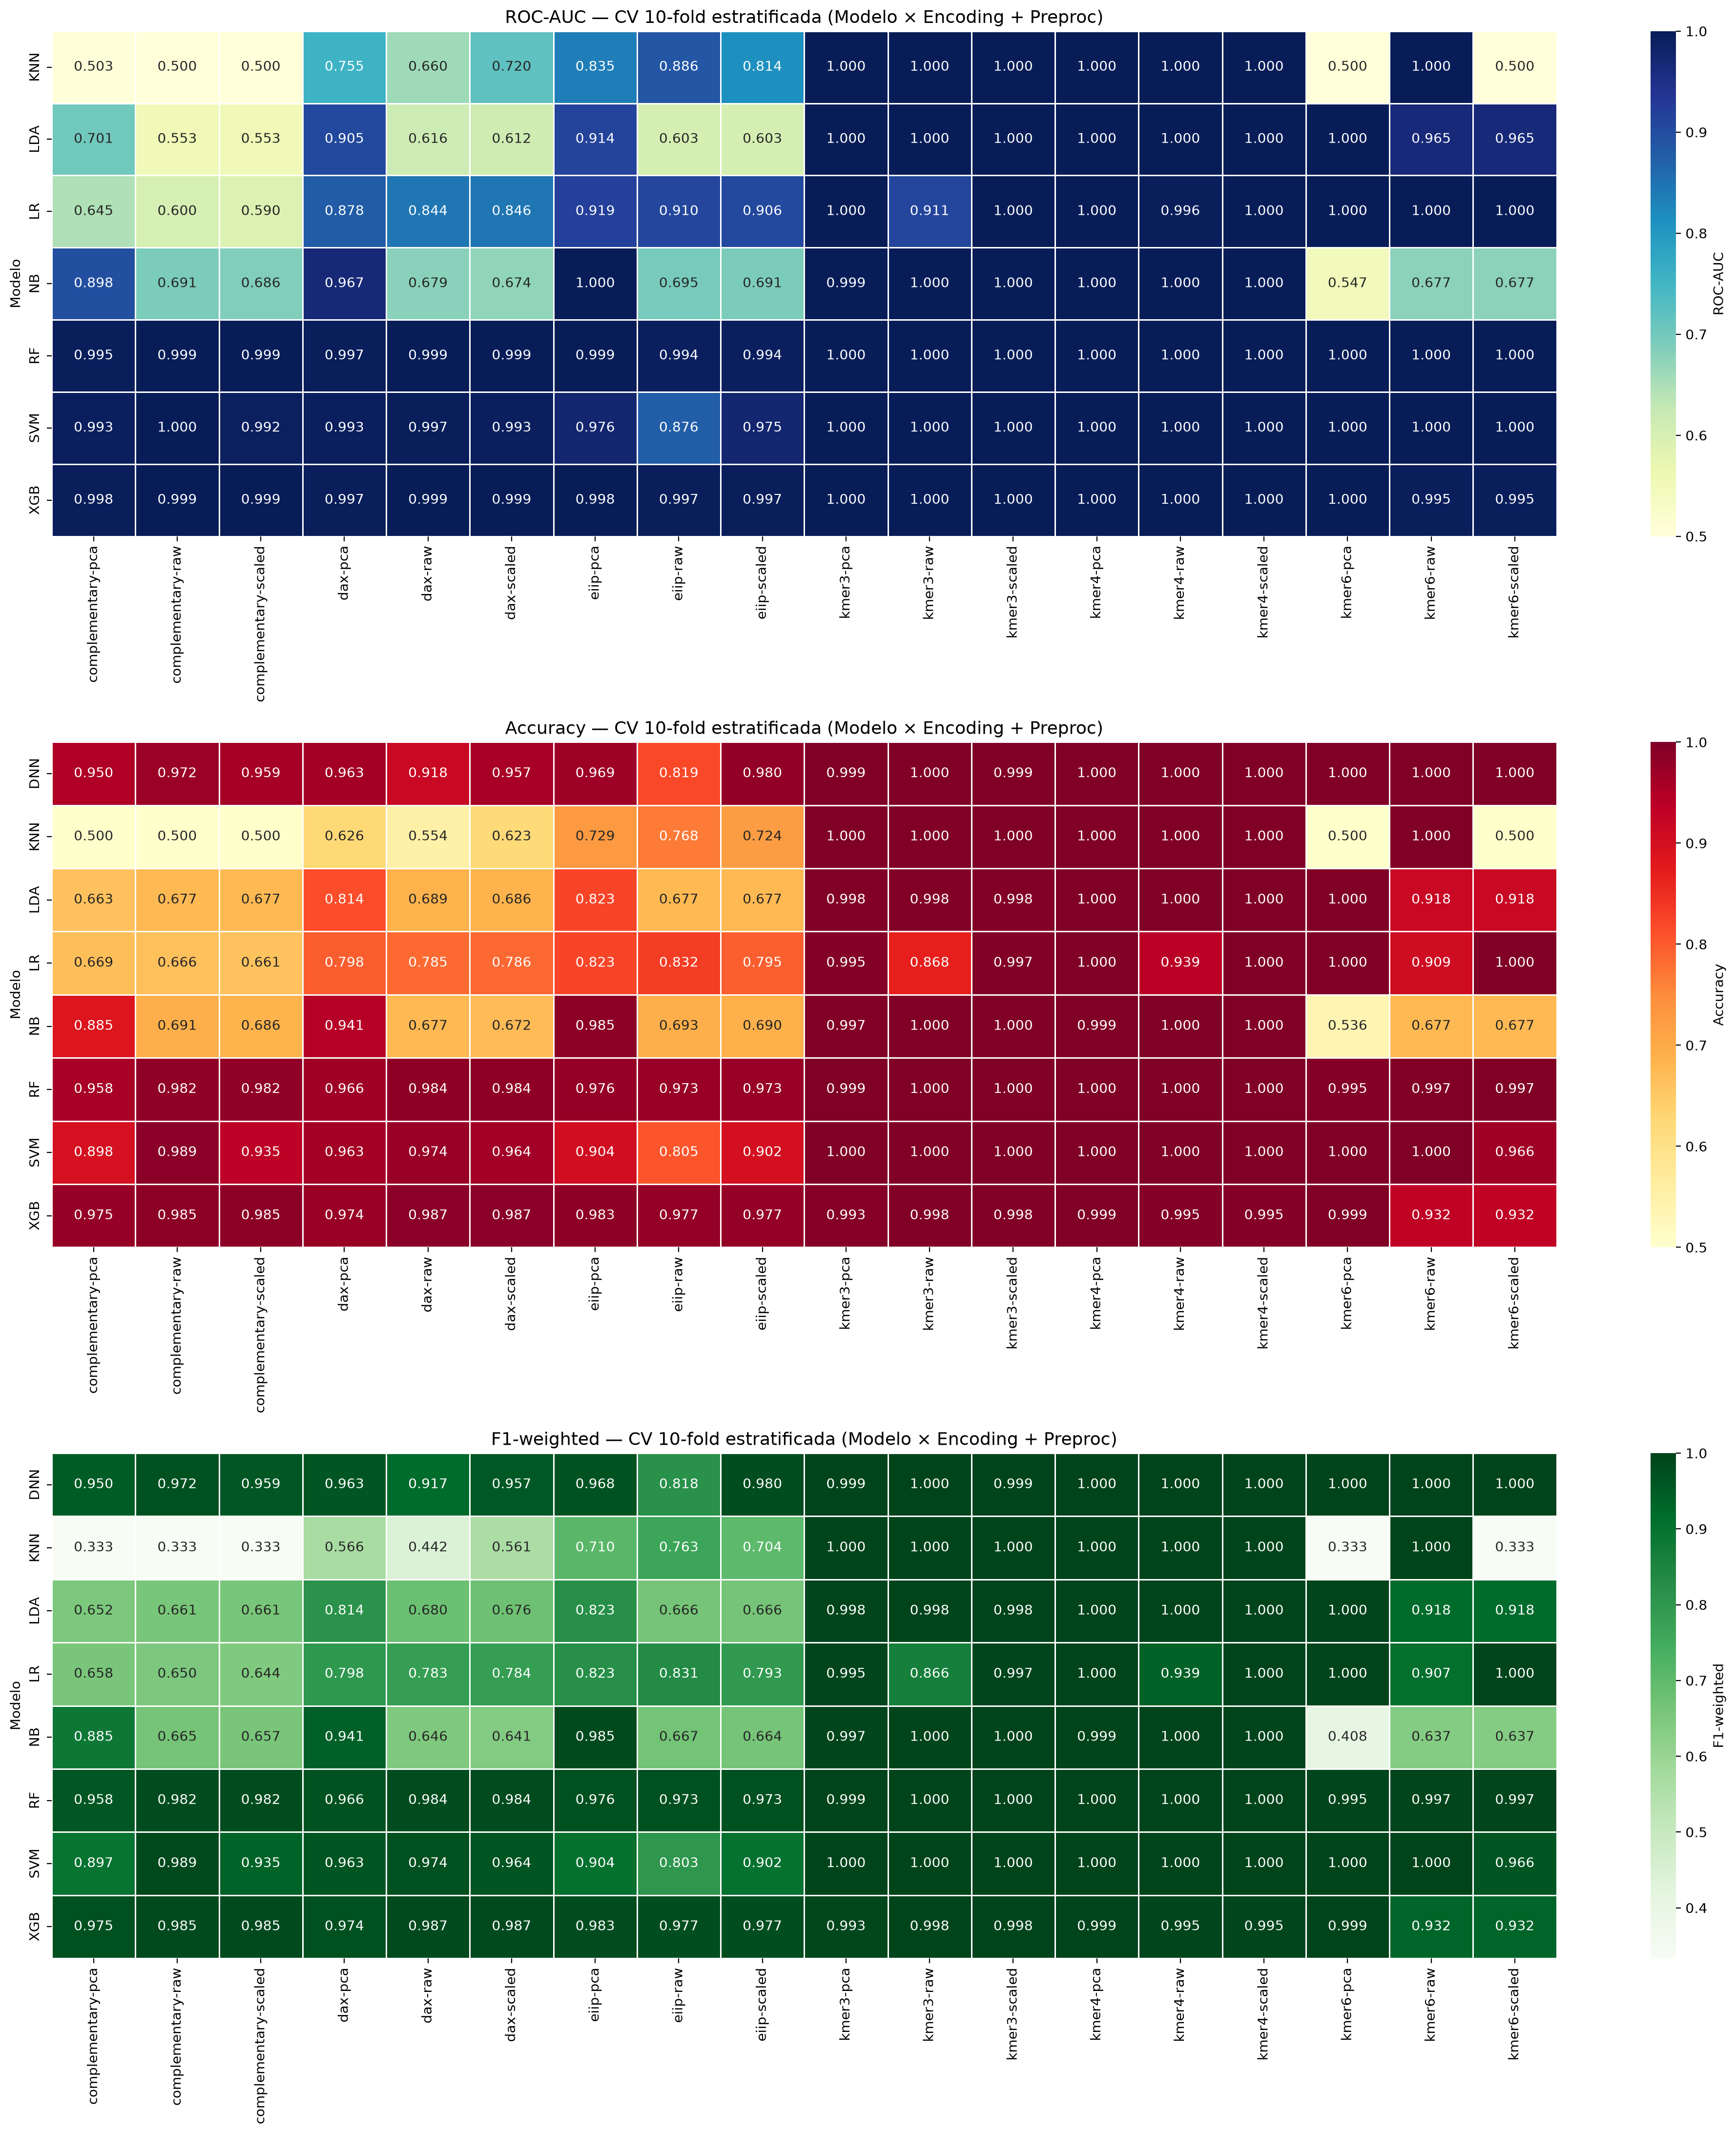
\includegraphics[width=0.98\textwidth,height=0.72\textheight,keepaspectratio]{fig1_heatmap_comparativo.png}
\caption{Mapa de calor comparativo (AUC, exactitud y F1 ponderado) de los ocho modelos a lo largo de
las seis codificaciones y los tres preprocesamientos, bajo validación cruzada estratificada 10-fold.
Las codificaciones por \textit{k}-meros (bloques de la derecha) concentran el rendimiento máximo.}
\label{fig:heatmap}
\end{figure*}

% ---- Figuras de una columna ----
\begin{figure*}[t]
\centering
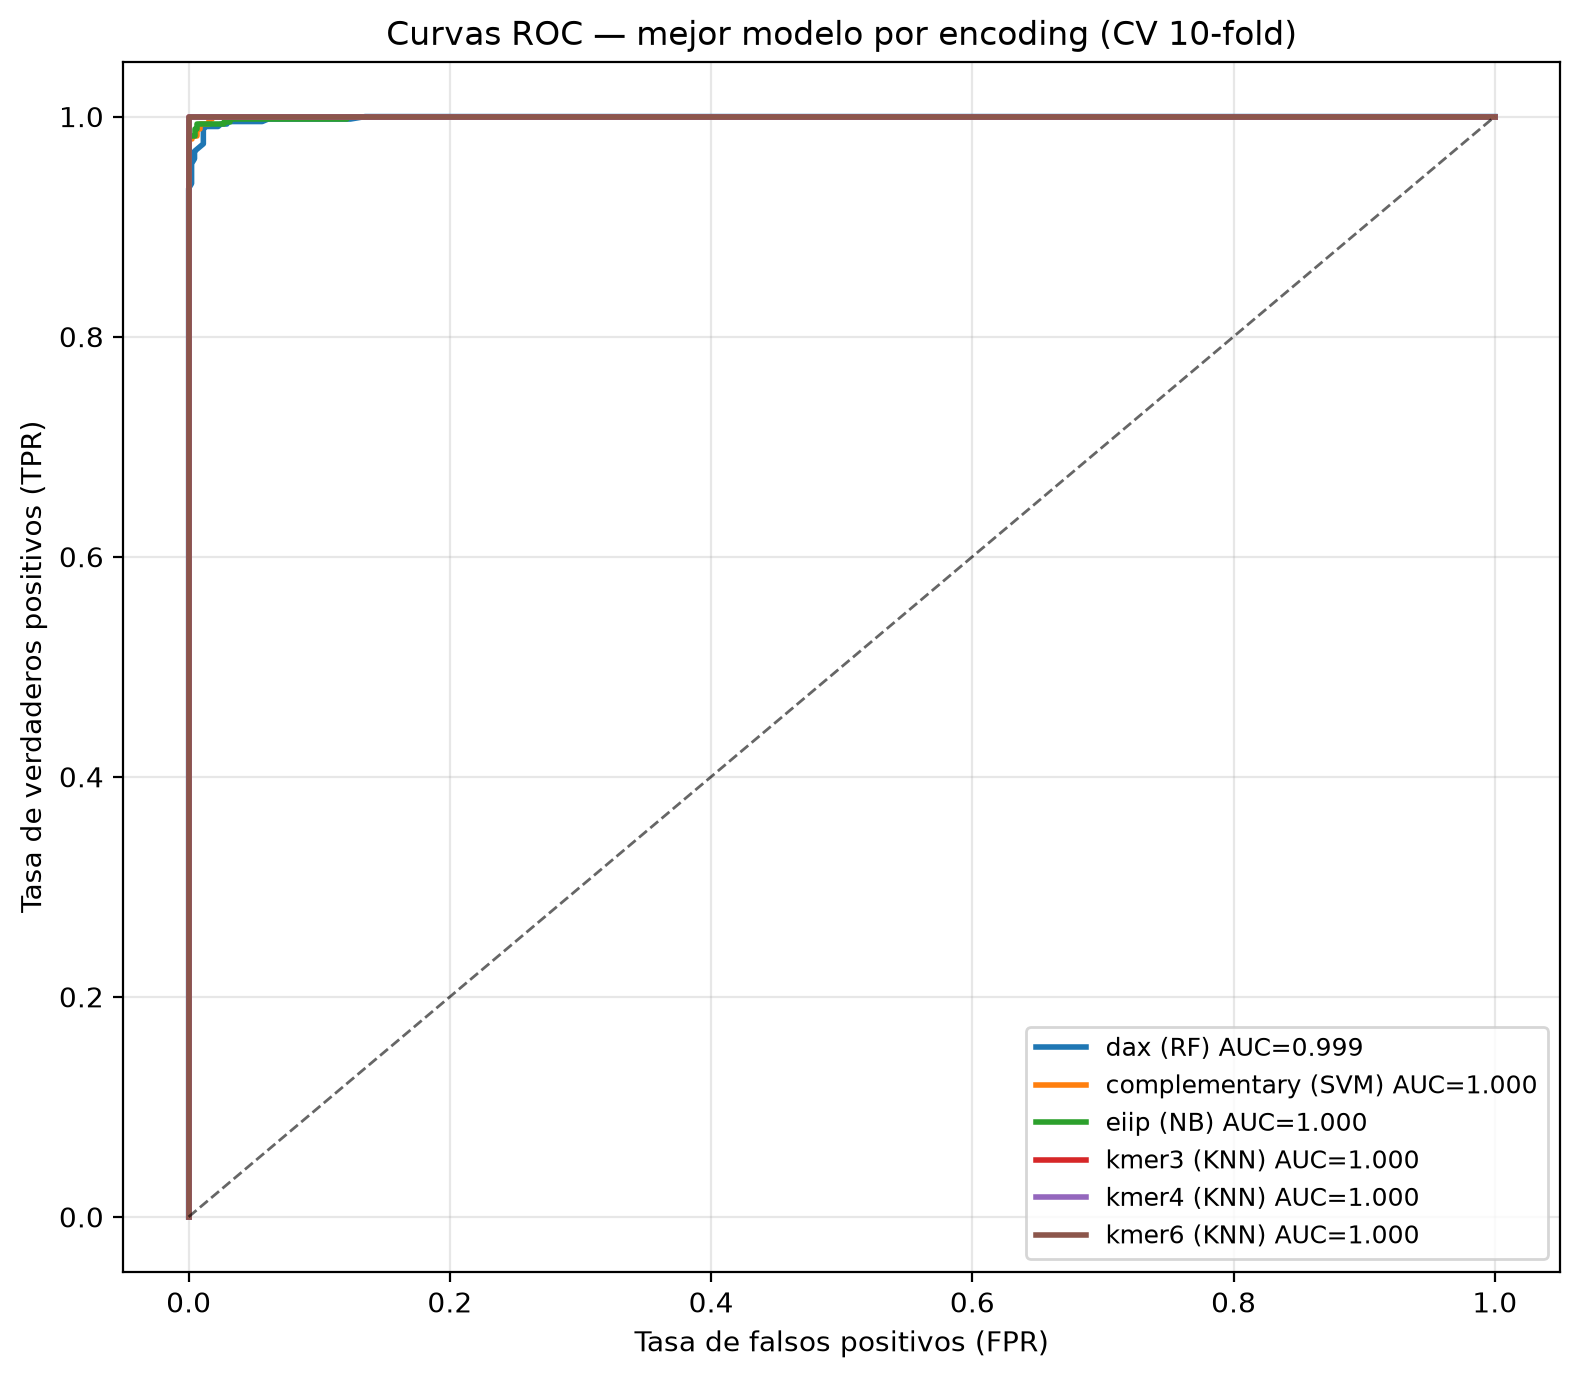
\includegraphics[width=\textwidth,height=0.5\textheight,keepaspectratio]{fig3_roc_por_encoding.png}
\caption{Curvas ROC del mejor modelo por codificación (CV 10-fold). Todas las representaciones por
\textit{k}-meros alcanzan AUC $=1{.}000$.}
\label{fig:roc}
\end{figure*}

\begin{figure*}[t]
\centering
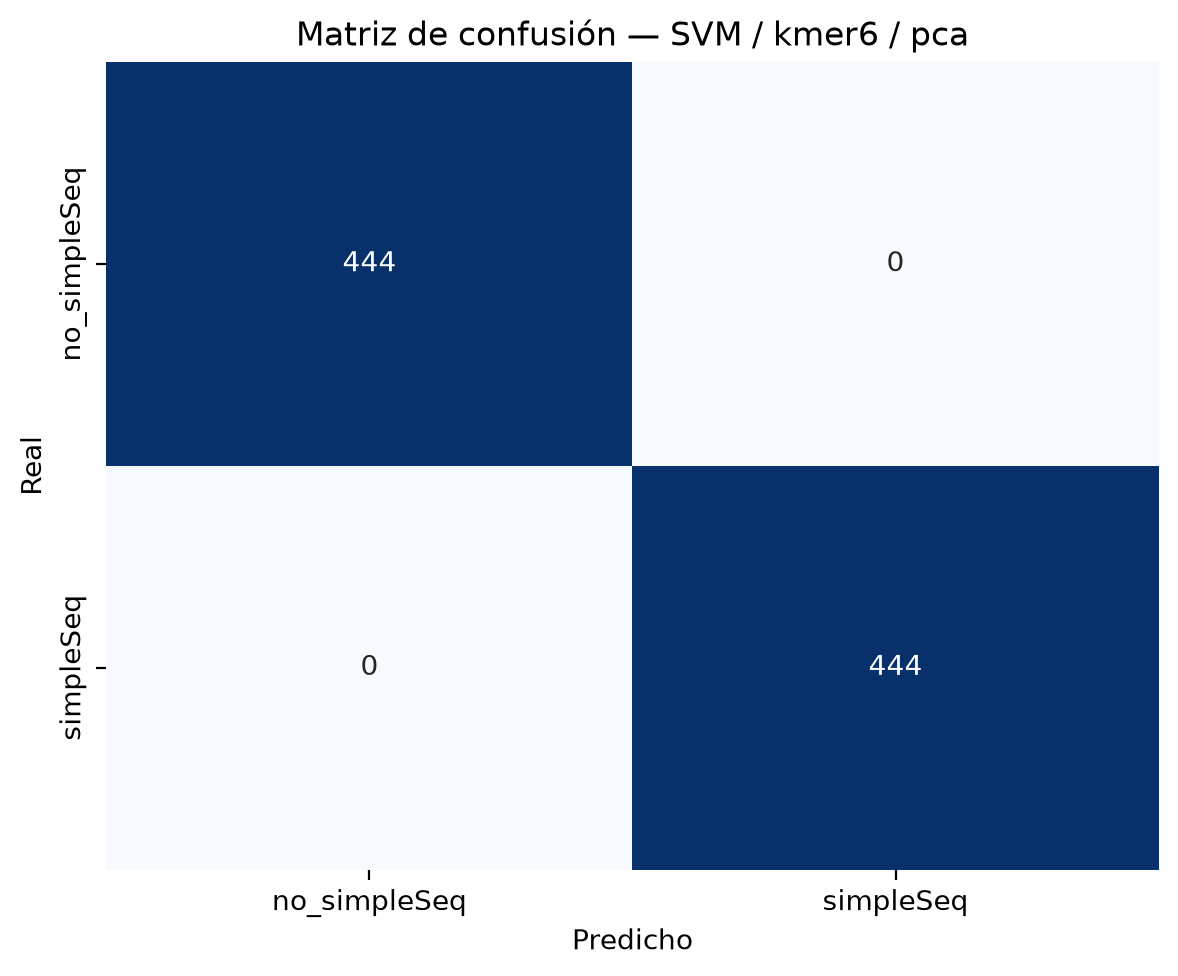
\includegraphics[width=\textwidth,height=0.5\textheight,keepaspectratio]{fig2_confusion_best.png}
\caption{Matriz de confusión de una configuración con rendimiento perfecto: 444/444 secuencias
correctamente clasificadas en ambas clases. El modelo desplegado (RF / \textit{k}-mer4 /
estandarización) produce la misma matriz con una fracción del coste.}
\label{fig:cmbest}
\end{figure*}

% ---- Figura ancha: CM de todos los modelos ----
\begin{figure*}[t]
\centering
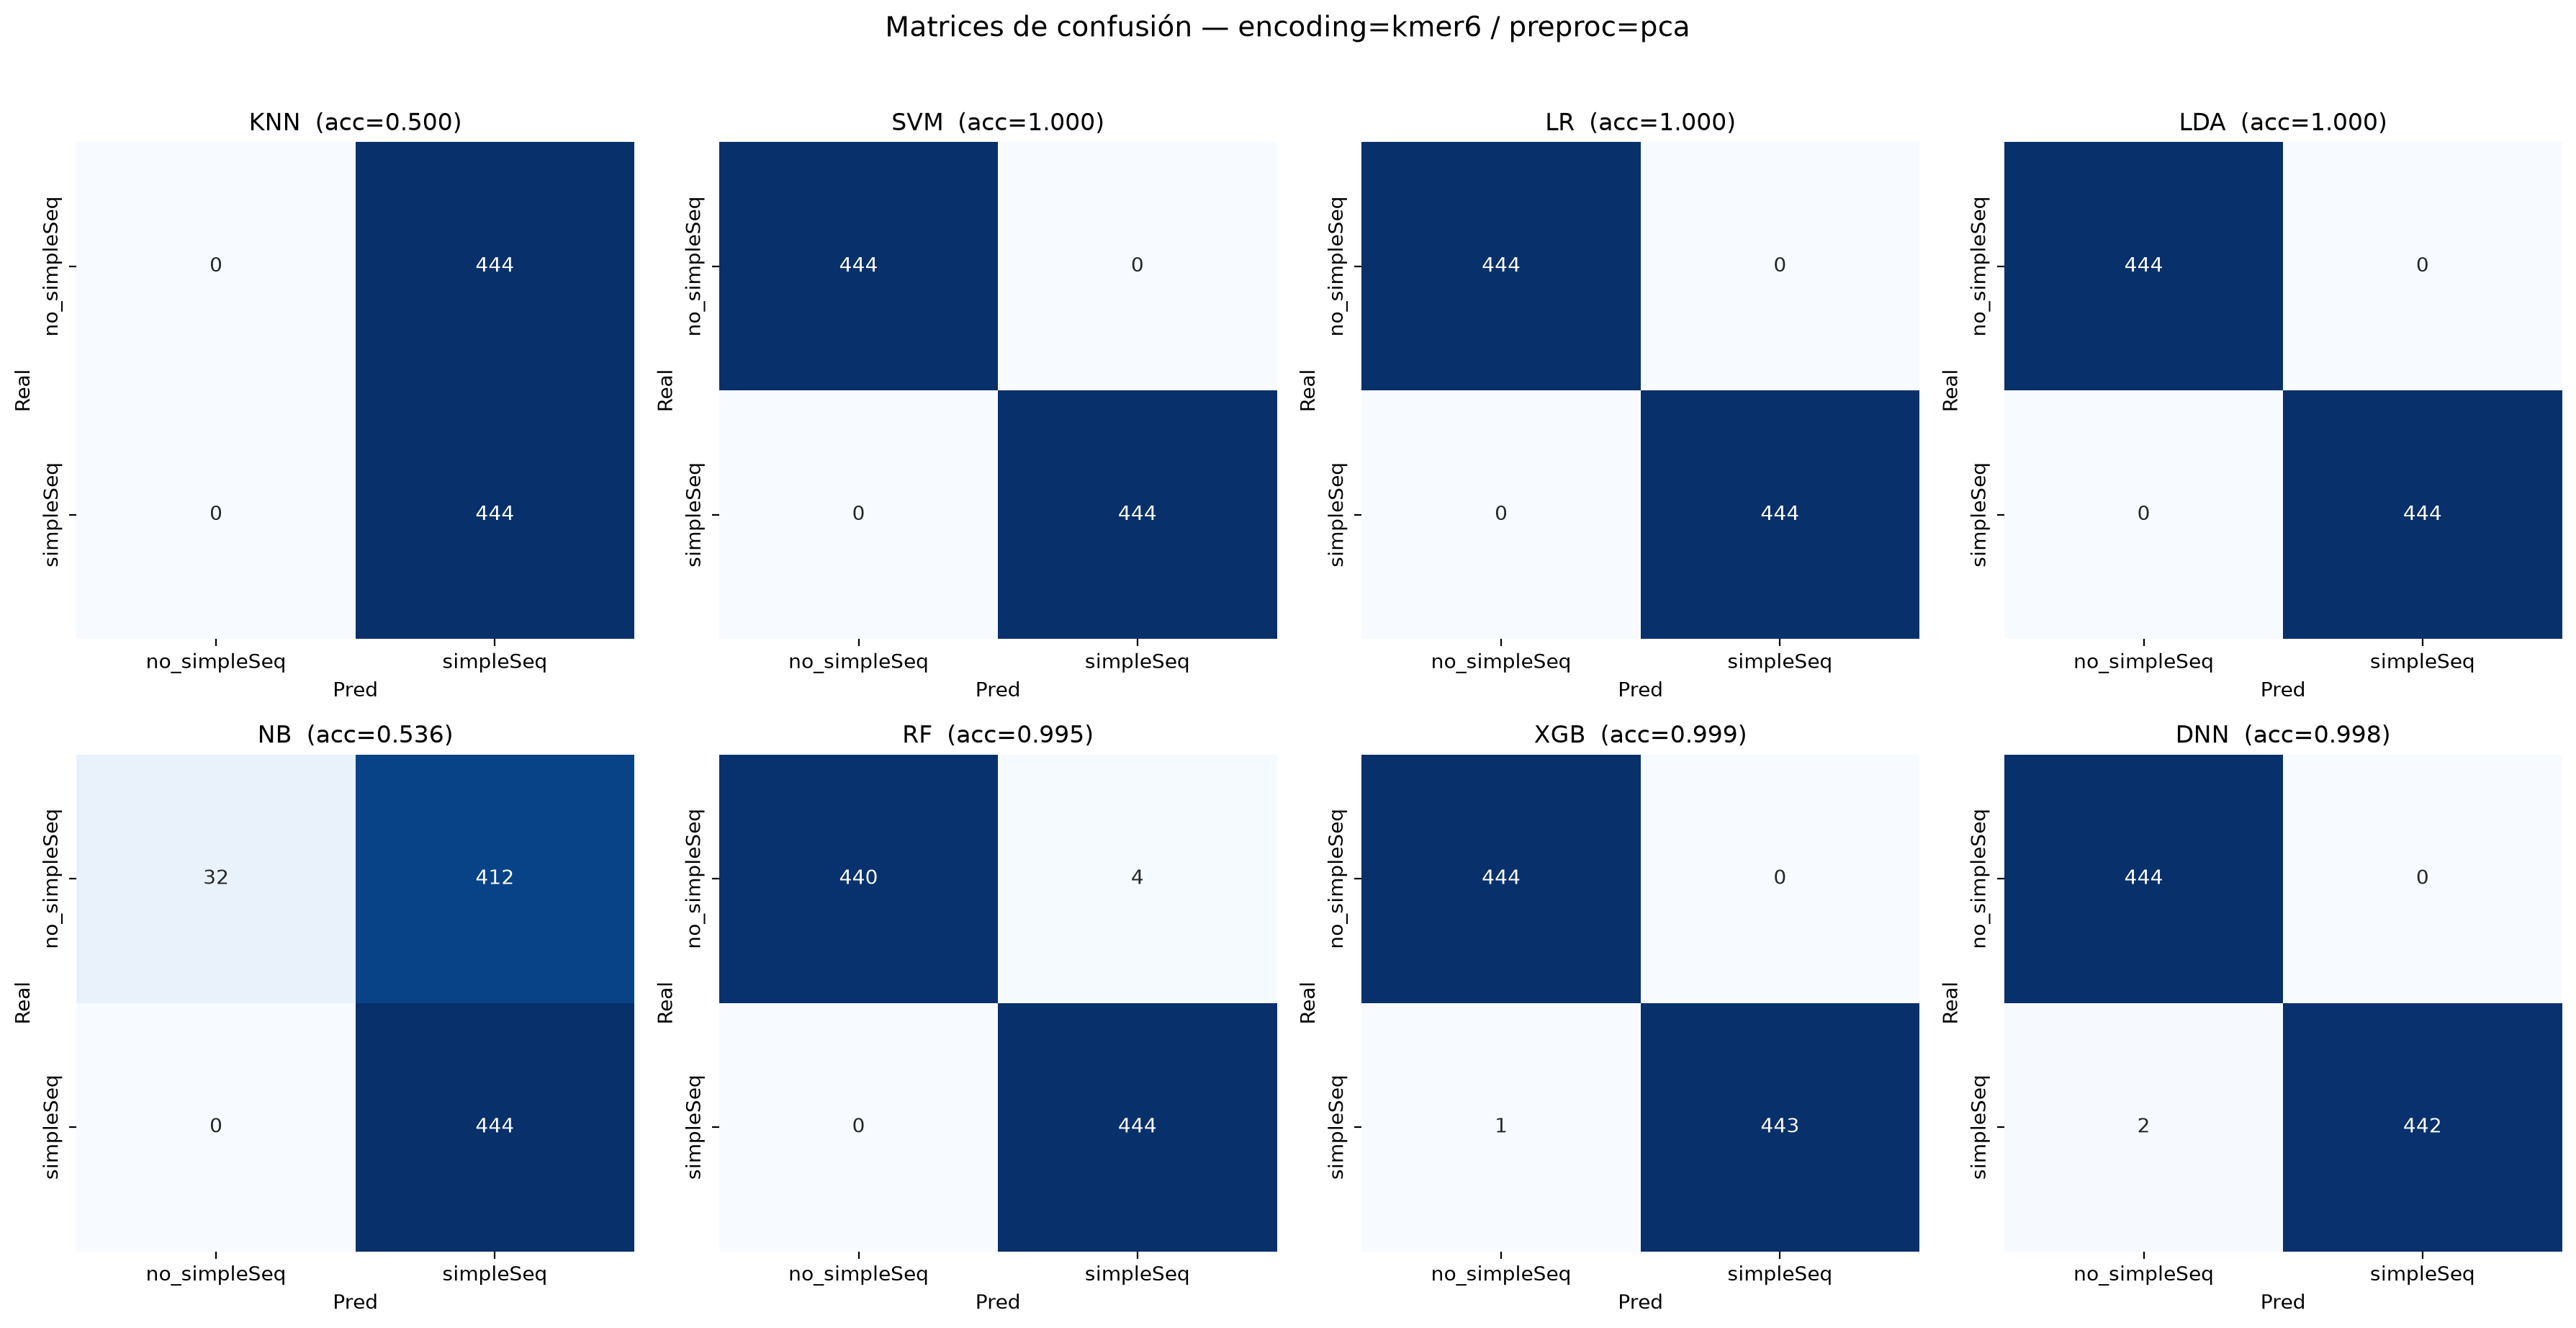
\includegraphics[width=\textwidth,height=0.42\textheight,keepaspectratio]{fig_cm_todos_modelos.png}
\caption{Matrices de confusión de los ocho modelos sobre la mejor codificación, mostrando el patrón
de errores de cada clasificador.}
\label{fig:cmall}
\end{figure*}

\begin{figure*}[t]
\centering
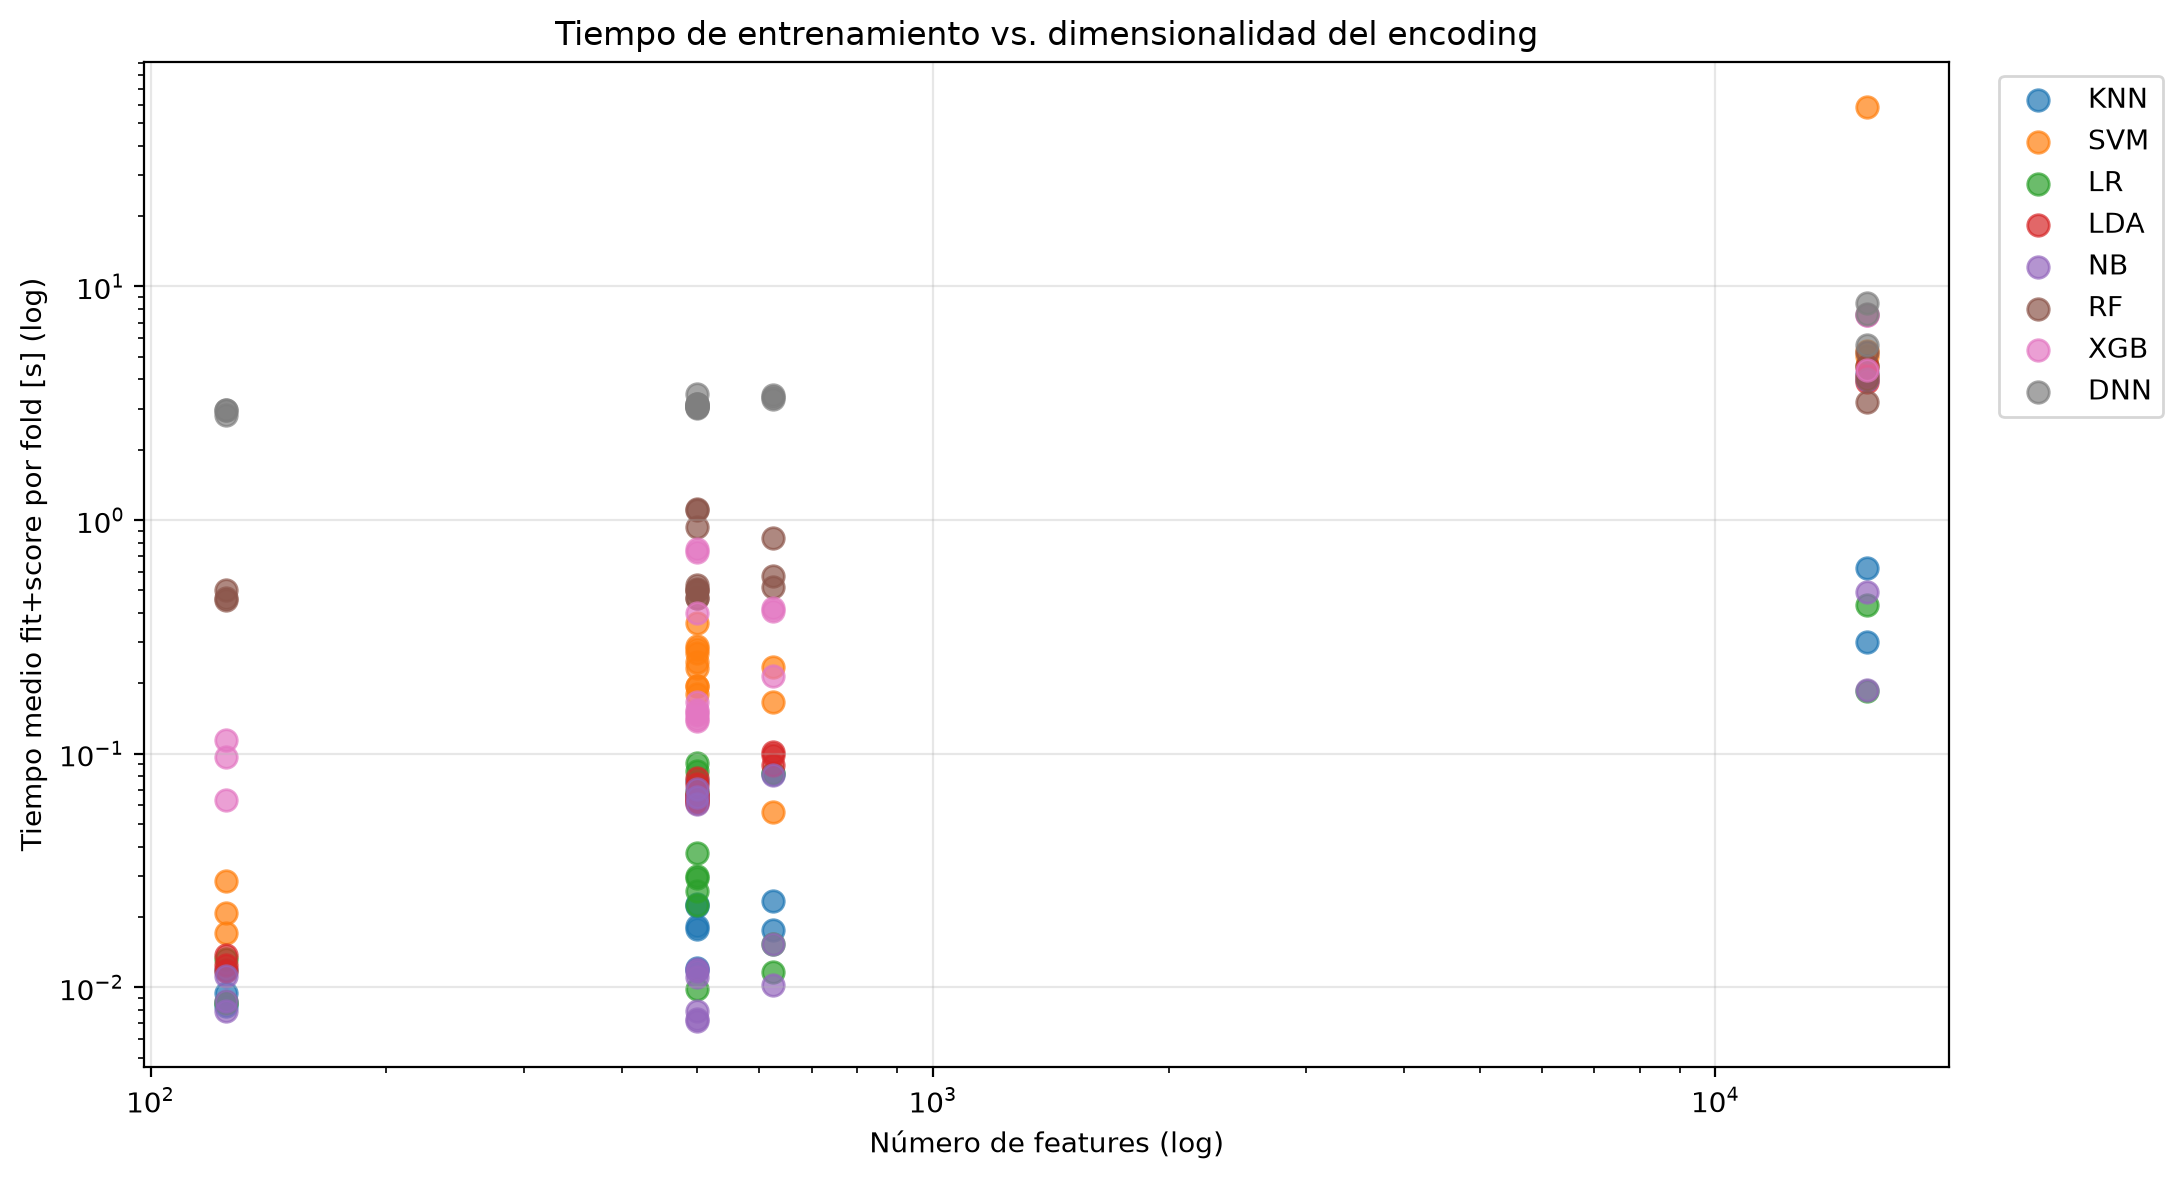
\includegraphics[width=\textwidth,height=0.42\textheight,keepaspectratio]{fig4_tiempo_vs_features.png}
\caption{Tiempo medio de entrenamiento por \textit{fold} frente a la dimensionalidad de la
codificación (ejes logarítmicos). El coste crece con el número de características; SVM sobre
\textit{k}-mer6 (15\,625 características) es el caso más costoso.}
\label{fig:time}
\end{figure*}

% =====================================================================
\section{Discusión}
% =====================================================================
La separabilidad casi perfecta de las codificaciones por \textit{k}-meros es coherente con la
naturaleza del problema: un \textit{simple repeat} se define por la \emph{periodicidad composicional}
de su secuencia, que la frecuencia de \textit{k}-meros captura de forma directa, mientras que las
codificaciones posicionales diluyen esa señal. Que un modelo tan simple como \textit{k}-NN sobre
\textit{k}-mer3 alcance el 100\,\% sugiere que, en este conjunto, las clases son linealmente
separables en el espacio composicional.

Esto constituye también la principal \textbf{limitación}: el conjunto es semi-sintético (composición
calibrada con datos reales pero secuencias generadas), por lo que los valores perfectos no deben
extrapolarse a datos genómicos reales sin validación adicional, donde se esperan fronteras de decisión
más difusas (repeticiones degeneradas, transiciones repeat/no-repeat, sesgos de secuenciación). Como
trabajo futuro proponemos validar sobre regiones anotadas reales, incorporar repeticiones imperfectas
y comparar contra TRF/RepeatMasker en datos genómicos. Para uso práctico recomendamos la configuración
parsimoniosa (\textit{k}-mer3/4 con un modelo de árboles), que combina exactitud máxima, bajo coste y
características interpretables.

% =====================================================================
\section*{Disponibilidad y requisitos}
% =====================================================================
\noindent\textbf{Repositorio:} \url{https://github.com/leandropa00/SimpleRepeatSeq}.\
\textbf{Lenguaje:} Python $\ge 3.9$.\
\textbf{Dependencias:} biopython, numpy, pandas, matplotlib, seaborn, scikit-learn, xgboost,
tensorflow$\ge$2.13, scikeras, joblib.\
\textbf{Instalación:} \texttt{pip install -r requirements.txt}.\
\textbf{Uso:} ejecutar \texttt{notebooks/01\_load\_data.ipynb} y \texttt{02\_experiments.ipynb}, o
clasificar un FASTA con \texttt{python classify.py --fasta entrada.fasta --model
models/best\_model.pkl --encoding kmer4}.

% =====================================================================
\begin{thebibliography}{99}
\small
\bibitem{benson1999} Benson G. Tandem repeats finder: a program to analyze DNA sequences.
\textit{Nucleic Acids Res.} 1999;27(2):573--580.
\bibitem{repeatmasker} Smit AFA, Hubley R, Green P. RepeatMasker Open-4.0. 2013--2015. Disponible en:
\url{http://www.repeatmasker.org}.
\bibitem{vinga2003} Vinga S, Almeida J. Alignment-free sequence comparison---a review.
\textit{Bioinformatics.} 2003;19(4):513--523.
\bibitem{wood2014} Wood DE, Salzberg SL. Kraken: ultrafast metagenomic sequence classification using
exact alignments. \textit{Genome Biol.} 2014;15(3):R46.
\bibitem{gymrek2012} Gymrek M, Golan D, Rosset S, Erlich Y. lobSTR: a short tandem repeat profiler for
personal genomes. \textit{Genome Res.} 2012;22(6):1154--1162.
\bibitem{breiman2001} Breiman L. Random forests. \textit{Mach Learn.} 2001;45(1):5--32.
\bibitem{chen2016} Chen T, Guestrin C. XGBoost: a scalable tree boosting system. En:
\textit{Proc.\ 22nd ACM SIGKDD Int.\ Conf.\ Knowl.\ Discov.\ Data Min.} 2016. p.\ 785--794.
\bibitem{pedregosa2011} Pedregosa F, Varoquaux G, Gramfort A, \textit{et al.} Scikit-learn: machine
learning in Python. \textit{J Mach Learn Res.} 2011;12:2825--2830.
\bibitem{cock2009} Cock PJA, Antao T, Chang JT, \textit{et al.} Biopython: freely available Python
tools for computational molecular biology and bioinformatics. \textit{Bioinformatics.}
2009;25(11):1422--1423.
\bibitem{tensorflow2016} Abadi M, Barham P, Chen J, \textit{et al.} TensorFlow: a system for
large-scale machine learning. En: \textit{12th USENIX Symp.\ Oper.\ Syst.\ Des.\ Implement.\ (OSDI).}
2016. p.\ 265--283.
\end{thebibliography}

\end{document}
